\documentclass{article} 
\usepackage[a4paper, margin=3cm]{geometry}

\usepackage{cite}
\usepackage{graphicx}

\usepackage{clrscode}

\title{Efficient Localised Heuristic for Influence Maximisation} 
\author{Antoni Zyla (u5527350) - Supervised by Nathan Griffiths}
\date{09/04/2026}

\begin{document}

\maketitle
\tableofcontents

\newpage
\section{Abstract}

Influence maximisation is the process of choosing a subset of population within a network to maximise the spread of an idea or concept under a certain model of propagation.
Computing the optimal solution is NP hard and therefore not feasible to compute for networks of a practical size.
Existing approaches including the greedy algorithm and it's optimisation produce a good theoretical guarantee as an approximation of the optimal solution but even still tend to scale poorly even on relatively small networks.
\\

In this paper we propose and evaluate an approach to efficiently solving this problem across three primary models of propagation, the independent cascade model, the decreasing cascade model and the linear threshold model.
We test across six (6) real world networks of varying topologies and scale, sampled using the Metropolis Hastings Random Walk with Delayed Acceptance (MHDA) algorithm, a performant and topology preserving method.
Statistical analysis is performed using Mann-Whitney U tests to determine equivalence of distributions, power tests to determine sample sizes and Cohen's d to measure effect sizes.
\\

Our proposed heuristic investigates locally computable node metrics in conjunction with network wide measures and metrics.
Performance of an approach is highly dependent upon different network topologies, starting influential set sizes and the underlying community structures of networks.
Our strongest performing heuristic is a combination of the degree of a node and the mean degree across it's neighborhood, it consistently matches or exceeds CELF across all of the networks under the decreasing cascade model and the linear threshold model at all seed sizes, using a 1000 seed network sample.
The ability to be computed with no global knowledge of the network makes it a very performant option which can scale across vast networks.
\\

We also investigate community based methods, attempting to exploit the properties of the greedy modularity maximisation community detection algorithm to capture influential nodes in an efficient manner.
\\

Our results suggest that simple and carefully constructed heuristics can reliably match the performance of a computationally heavy approximation method across a range of real world network topologies.
We find community based methods perform very well as shown in literature but we are unable to make gains past that.

\newpage
\section{Introduction}
If we were a marketer with access to a population of people and some information about the relationships between them, we may choose a subset of this population who would most effectively market our product.
We can consider a population of people in a graph as nodes with relationships between them as edges.
Using a model of concept spread we can choose a subset of nodes to act as seeds from which ideas propogate, they may have a direct chance of propagating to their neighbors or another non direct effect.
\\

Choosing an optimal subset of the population that will produce the greatest influence spread is an NP hard problem via a reduction from set cover.
Approaches such as the Greedy algorithm and it's optimisation CELF (Cost Effective Lazy Forward) produce a very good theoretical approximation of $(1-1/e)$ of the optimal result (this is approximately 63\%).
Despite being well optimised these approaches take a very long time to compute, up to thousands of times longer than very simple heuristics.
\\

Real world networks may have tens or even hundreds of thousands of nodes with millions of edges between them.
Even CELF may be far too slow to operate on such a scale despite being approximately 700 times faster than a naive greedy approach.
Approaches requiring knowledge of the entire network to compute some measure about a node may also become unfeasible to compute on such networks.
Finding lightweight approaches is therefore crucial to efficient influence maximisation in larger networks.
Degree based methods have been shown to be highly effective across a range of networks as they exploit the scale free property of typical social networks in which the majority of influence is held by few nodes.
Community based approaches aim to exploit the typical clustering of nodes into dense communities with ties inside the communities and poor ties between nodes in different communities to work in a divide and conquer manner by aiming to saturate communities and identify nodes which are key links between communities.
\\

We find that a single lightweight heuristic, made by giving each node a score of the ratio of their degree to the mean degree of their immediate neighbourhood is able to outperform CELF across each network topology under the decreasing cascade model and the linear threshold model.
We also investigate methods used in community detection or partitioning of networks to find influential nodes.

\newpage
\section{Literature Review}

\subsection{The Influence Maximisation Problem}

\textbf{Definition: Influence Maximisation Problem} Given a network $G = (V, E)$, a non negative integer $k$, and a model of propagation $M$.
\begin{itemize}
	\item Find the subset $S \subset V$ of size $k$ such that the expected spread through $G$ under the model $M$ with $S$ as the starting seeds is maximised.
\end{itemize}

\subsection{Why is it NP-Hard?}
Under a given influence influence model choosing the optimal starting set is an NP-hard problem.
We can prove this using a reduction from a known NP hard problem, Set Cover.

\vspace{1em}
\noindent \textbf{Definition: Set Cover} Given a universe of elements $U$, a set of subsets of $U$, $S = \{S_1, S_2, ..., S_m\}$, and a non negative integer $k$.
\begin{itemize}
	\item Return True if there exists $S' \subset S$ where $|S'| = k$ and $\cup S' = U$
	\item Return False otherwise
\end{itemize}

Given an instance of set cover with a universe $U$, a collection of subsets $S = \{S_1, S_2, ..., S_m\}$ and a non negative integer $k$.
We can construct a bipartite graph $G = (A \cup B, E)$ where $A$ contains one node for each subset in $S$. $B$ contains each element contained in the universe $U$. The edges between the set of nodes $A$ and $B$ are contents of each of the subsets contained in $S$.

Using a model of influence where a node has a probability of 1 to infect it's neighbours, and a limit of only going 1 hop across.
\\

\textbf{Claim} There exists a set cover of size $k$ iff there exists a seed set of size $k$ which covers a total of $k + |U|$ nodes.
\\

Set Cover implies IM: If there exists a set cover of size $k$ then choosing the corresponding nodes within the set $A$ will infect every node in $B$ as they are a direct mapping of the sets. This will produce a coverage of $k$ nodes in $A$ and all of $U$ satisfying the claim.
\\

IM implies Set Cover: If there exists a seed set of size $k$ which achieves $k$ + $|U|$ then every node in $B$ must be activated. All seeds must come from the set $A$, if our set contained a node $b$ from $B$ then we could directly substitute $b$ for any of it's neighbours in $A$ as they will infect not only $b$ but also all of their other connections. The influence from $b$ would only be able to infect one node in $A$ and then stop due to the limit of 1 hop. The chosen nodes must cover every node in $B$ meaning that the corresponding subsets cover every node in $U$ solving set cover \cite{tardoskempe2003}.

\subsection{Models of Influence Propagation}
We will be focusing on three (3) main methods for influence spread across networks.

\begin{enumerate}
	\item Independent Cascade Model (IC) \cite{tardoskempe2003} - Each node can take a state out of Active, Inactive and uninfected.
	      Each active node has a probability $p$ to infect each of it's uninfected neighbors.
	      Once a node has been infected this process starts again to all of it's neighbors, the node is in the active state once it is infected \cite{tardoskempe2003}.
	      Once a node has attempted to infect all of it's neighbors it becomes an inactive node.
	      This is the simplest of the models but also mimics real life well, whether it's the spread of a new software technology or a new restaurant becoming more popular.
	\item Decreasing Cascade Model (DC) - A modification of the ICC model where every attempt of a node to be influenced decreases the probability of it being influenced or infected \cite{kempe2005influential}.
	      This could be analogous to a common experience, overreaching of advertisements or correspondence, such as marketing emails which have the opposite to intended effect due to annoyance.
	\item Linear Threshold Model (LTM) - Every node $v$ is given a probability of being turned $p$ which is uniformly distributed across the interval $[0, 1]$. When the proportion of node $v$'s neighbors which are infected is greater than or equal to $p$, $v$ itself becomes infected \cite{tardoskempe2003}.
	      This models well another common experience, a group reaching a common view in regards to something, whether it's the adoption of a new game, or even a software tool that becomes the 'industry standard' this principle is at play.
\end{enumerate}

Various papers have described modifications of each of these models in a multitude of ways, multiple concepts can be spread wherein they can inhibit the spread of eachother by allowing a node to only adopt a single concept \cite{griffiths17LimitiingConcept,goyal2012competitivecontagionnetworks}.
Vaccination or herd immunity can also be modelled in this manner \cite{griffiths17LimitiingConcept}.
\\

There are other models which work in different manners, borrowing from biological models such as SIR (Susceptible-Infected-Recovered) for modelling diseases more closely \cite{kuperman2013invited}. These are somewhat able to be modelled using the cascade models described however full parity is not possible.
A node going from infected to uninfected is not a behavior that is considered within the cascades and would possibly have large effects on the effectiveness of certain seed selection strategies.
It is possible to take an agent based approach to influence giving each agent certain characteristics as used in \cite{archbold2024cvd} for modelling behavioral risk factors of cardiovascular disease spreading across city scale populations.
\\

Developed in 2008 the heat diffusion model (HDM) works on a similar principle to the linear threshold model to model the spread of influence in social networks as accurately as possible.
The network has a parameter $\alpha$ which controls the rate at which heat flows between nodes, each node is given a threshold $\theta$ which is the minimum 'heat' required for it to become active.
The model also has a limit on how long it will run for a period of time $t$.
The rate of heat flow between two nodes is determined by the difference in heat and the value of $\alpha$, the more nodes are connected to a node spreading heat faster it will be conducted.
\\

Social Networks are constantly evolving systems.
Nodes are constantly added or removed, connections between nodes are frequently added, removed or rerouted, working on a snapshot of an ever evolving network may not be the most effective method for precise real world modelling.
Dynamic models of influence are models where paths between nodes can be added or removed as part of the process \cite{sekara2016fundamental}, this can for example be used to model the evolution of social networks, and how influential nodes may become more or less influential based on different factors or topology, rather than studying networks which are at a fixed point in their evolution.
\\

Another way in which this field has evolved is the study of adversarial contagions.
Analogous to the spread of a disease against a vaccination, two concepts/contagion spreading across the network at the same time \cite{griffiths17LimitiingConcept}.

\subsection{Working with large networks}
Sampling networks is a way of preserving the topological features and general properties of a network whilst giving us smaller networks to allow for easier computation.
This allows us to create strategies by quickly testing on small networks to see what works and what doesn't and then we can generalise our approach to larger networks .

\subsubsection{Naive Approaches}
A simple natural approach could be to take a node at random from the graph, call it $v$, and then perform a breadth first search in layers across the graph.
An issue with naive BFS is that when a high degree node is encountered then each of it's neighbours would also be added, this will inflate the average degree of the network by tending to sample a subset with a higher mean degree \cite{Wang2011UnderstandingGS}.
\\

Working outwards from a start node does not preserve the distribution of shortest path distances between nodes or clustering coefficients well.
Nodes close to the root will maintain accurate values but as we move further and further out a node is less likely to appear before we have no more nodes needed leading to a lower shorter mean path length and a higher clustering coefficient over other methods \cite{gjoka2010}.
Some papers describe BFS as adding the entire layer from which it explores, leading to oversized samples \cite{franks2014learning}.
Taking a BFS sample of 1000 nodes in the Enron dataset can produce a subgraph of over 12 thousand nodes which is not comparable to a standard 1000 node sample.
\\

It is important to compare like for like network sizes, topological features such as diameter, maximum degree or mean shortest path length are closely dependant on overall network size.
\\

Snowball sampling is a variation on breadth first search,
once the addition of the final layer would take the total number of sampled nodes over the sampling threshold, nodes are added one at a time until the exact number of nodes is reached \cite{franks2014learning}.
\\

A random walk is another simple strategy for exploring a graph.
Working on the basis of a standard random walk, starting from a node $v$ there is a $\frac{1}{deg(v)}$ probability of choosing the next node to be $u$ where $u$ is one of the neighbours of $v$.
A random walk based approach will suffer from the same problems as BFS with finding higher degree nodes much more often than lower degrees \cite{gjoka2010}, as a higher degree node has more connections that lead to it.

\subsubsection{Smarter Sampling Methods}
Utilising modified random walks is a standard method of achieving accurate and unbiased samples of large networks such as facebook \cite{gjoka2010}.
Metropolis Hastings Random Walks and Random Walks with Delayed Acceptance (MHRW and MHDA) are two common methods used \cite{gjoka2010, gjoka11practicalreco}

\begin{enumerate}
	\item Metropolis Hastings Random Walk (MHRW) - Sample a random uniform probability in the range 0 to 1 and call it $p$. We add a node if for a given node $p \leq \min\{1, \deg{x_0} / \deg {x_1}\}$ where $x_1$ and $x_0$ are nodes that we are selecting during the process of our random walk \cite{gjoka2010}. This produces representative samples of the network.
	\item Metropolis Hastings Random Walk with Delayed Acceptance (MHDA). This is a further modification of MHRW where nodes with a high degree are less likely to be chosen with a reduction in backtracking \cite{lee2012randomwalkmetropolishastingssamplers}.
	\item Albatross Sampling (AS) - A random walk based sample with a probability of jumping to a random node within the network, this should allow for better capture of networks with disconnected or densely clustered components or communities on a very large scale \cite{jin2011albatross}.
\end{enumerate}

\subsubsection{Scale Free Networks}
A scale free network is one where the distribution of individual node degrees could be modelled using an exponential function.
In this case the probability of a node having a degree $k$ is modelled by the below equation \cite{satorras2008scalefree}.

\begin{equation}
	P(k) \sim k^{-\gamma}
\end{equation}

There exist few nodes with a very high number of connections with the majority of nodes having a low number of connections.
Some examples of scale free networks are typical human social networks.
A simple way to visualise this is by looking at your facebook or instagram account, you and the majority of people may on average have maybe 20-50 friends or connections, checking the numbers of an actor or influential figure may yield values in the millions.
\\

If a large proportion of the network is able to quickly reached by these very high degree nodes then this informs that the value of a degree based heuristic may prove to be more valuable than any other heuristic \cite{tardoskempe2003}.
In contrast networks that do not exhibit this behaviour are often not as easily spread through using basic heuristics.
Utilising community based heuristics or more complex methods may be more worthwhile for such networks.

\subsection{Finding seed nodes}
There are a few methods which don't rely on a heuristic to determine the seed nodes.

\begin{enumerate}
	\item Brute Force, for a graph made up of $n$ nodes there are $n$ choose $k$ possible sets of starting seeds. Running a cascade for each of these would be incredibly inefficient and impractical by being on the order of $n$ factorial. I have not been able to find reference of this being used to compare with other methods likely due to the required processing power.
	\item Greedy, starting with an empty seed set choose the node in the subgraph of the network bar our seeds which will produce the largest influence, add this node to our set of seeds and continue to add nodes until we have a set of our desired size. This achieves a $1-1/e$ approximation ratio to the optimal solution due to exploiting the sub-modularity of additional nodes being added to the overall spread of ideas \cite{tardoskempe2003}.
	\item Cost Effective Lazy Forward (CELF). A modification of the greedy algorithm to prevent recomputation of the expected gain for each node by keeping a sorted heap of the marginal gain for each un-included node and only recomputing when the node at the top of the heap is no longer the optimal choice. This is up to 700 times faster than the greedy algorithm described above \cite{celf}.
\end{enumerate}

Other factors which can help us gauge how influential a node may be with no global knowledge of the graph required are:
\begin{enumerate}
	\item Degree (Deg). In the ICC and DCC models a node has some chance $p$ of spreading a concept to it's neighbours it is clear that on average it would spread to an expected $p \deg(v)$ nodes.
	      Likewise on threshold based models a high degree node being chosen will increase the proportion of infected nodes for it's very high number of neighbours triggering a likely large cascade \cite{tardoskempe2003}.
	\item Degree Discount (DD). It's known that high degree nodes tend to cluster together, choosing multiple tightly coupled high degree nodes is redundant and not as effective as it could be. Removing any neighbours of a selected node and then using degree is an effective way of minimising the overlap of expected influence between chosen seed nodes \cite{franks2014learning}.
	      Requiring a factor of $\Delta$ more computation power than raw degree heuristic it is a performant option.
	      There is a limitation with regards to networks which have a few very high degree nodes, by choosing just a few of these nodes there are often minimal nodes left to choose from and an appropriate sample is not able to obtained.
	\item Mean Neighbour Degree (MND). Thinking about how the cascade will propogate, choosing nodes who's neighbours are very high degree nodes will result in gaining access to multiple influential nodes (those with high degree) from a single seed \cite{franks2014learning}.
	      Compared to raw degree this requires a factor of $\Delta^2$ more computation. For most graphs this is still a very performant option as those very high degree nodes are very rare.
\end{enumerate}
Those above are quick to compute and importantly required no global knowledge of the network.
\begin{enumerate}
	\item Local Clustering Coefficient (LCC). Consider a node where each of it's neighbours is connected to every other neighbour, this would be a clique and a very highly clustered node. We are measuring how close a node is to being in a clique from it's neighbours by taking the proportion of neighbours connected to other neighbours from the total possible number.
	      Computing this is relatively fast being on average the mean degree cubed. Performance is dependant upon network topology. On a very simple level a highly clustered node will perform well at spreading concepts in it's immediate vicinity \cite{franks2014learning}. There are some cases where it may not be of use, if in a graph there exists a small almost unconnected clique of nodes of size greater than our seed size then choosing them all will not produce a good spread in the rest of the graph.
	      We compute the clustering of a node $v$ using the below equation.
	      \begin{equation}
		      C(v) = \frac{2 T(v)}{\deg(v)(\deg(v) - 1)}
	      \end{equation}
	      Where $T(v)$ is the number of triangles around the node $v$ \cite{clustering_coef}.
	\item Betweenness Centrality (BC). The proportion of shortest paths from any two nodes in the network which pass through the point. Take a graph of two communities with a single edge between them, the two nodes on either side of the edge would have a very high betweenness as they are vital for the connection of the two communities. Most topologies will not exhibit this extreme a distribution in betweenness however it is still a useful metric for influence. As we need to compute the shortest path between each pair of nodes there this is a very expensive heuristic on the order of $O(nm)$.
	      We calculate the betweenness of a node using:
	      \begin{equation}
		      B(v) = \sum_{s, t \in V, s \neq v \neq v} \frac{|\sigma(s, t | v)|}{|\sigma(s, t)|}
	      \end{equation} where $\sigma(s,t)$ denotes the set of shortest paths from node $s$ to $t$, with the conditional on $v$ is shortest paths which include $v$ \cite{betweenness}.
\end{enumerate}

\subsection{Community Based Methods}
Social networks typically have a natural community structure whether it's families, workplaces or schools it is feasible to partition a network into a set of communities which span the whole network.
Nodes within a community are strongly connected with links between communities being minimal \cite{cim}.
Working on the idea that if a community is isolated from the rest of the network then determining the expected influence of a node within it's community is a good indicator of it's global influence.

Though not working on the diffusion models we are targeting, instead on the heat diffusion model (HDM),
Introduced in 2014 by Chen et al, Community-Based Influence Maximization (CIM) model works in three phases, partitioning networks, determining nodes which should be used to select seeds and then choosing the exact selection of seed nodes \cite{cim}.

CIM works in three phases
\begin{enumerate}
	\item Partition the network into communities using h clustering. Nodes can be identified as hubs or outliers.
	\item Generate a set of nodes from which to choose our seeds. Considering only nodes which are hubs (connecting two communities), High degree and high similarity nodes within significant (communities larger than the expected spread from a single node) communities. It was found that just 10 percent of each significant community is enough to get worthwhile seed nodes.
	\item Seeds are chosen from each community and split up based on the size of the community to allocate more seeds to larger communities.
\end{enumerate}

The modularity of a network is a measure of how strongly split into communities the network is.

\begin{equation}
	Q=\sum _{i=1}^{c}(e_{ij}-a_{i}^{2})
\end{equation}

where $e_{ij}$ is the proportion of edges connecting communities $i$ and $j$, $a_i$ is the fraction of ends of edges which end in community $i$.
The value of Q determines how strong this community structure within a network is with values of around 0.3 representing a meaningful community split \cite{clausetnewman}.

If a network displays a strong community structure then that implies there exist subsets where it is hard for ideas to propogate between them.
If you were to choose nodes in just a single community then you might be able to saturate a community with a concept \cite{cim}, however this may not provide an optimal global spread of the concept in the network.

In certain scenarios this behaviour may be a good thing, if a community structure was very distinct and you wanted to for example use different strategies in different communities based on some type of underlying difference in structure or properties.

\subsubsection{Community Detection Algorithms}
The Girvan-Newman algorithm introduced in 2002 works on the basis of identifying edges which link communities \cite{girvannewman}.
In the same way that a node can have a betweenness coefficient so can an edge, finding the edges with the highest betweenness (or being critical choke points for connecting sets of nodes).
To find communities we can iteratively remove edges from the network until we have found the number of distinct communities \cite{girvannewman}.

In 2004 it was found that there exists a more efficient algorithm for community detection in networks based on the notion of maximizing modularity from combining communities using a greedy method \cite{clausetnewman}.
Starting with each vertex as it's own community, combine vertices to maximise the gain in modularity for the whole graph. Continuing to change the community each vertex belongs to until you cannot increase the modularity of the graph further.

\subsection{Evaluating network topology}
As a network is a graph made up of nodes and edges it's obvious to consider the number of nodes and edges or how these edges are distributed between the nodes.
There are many metrics we can use to gain an insight into the type of network topology we are working with.

\begin{enumerate}
	\item Diameter - The length of the longest shortest path from any two nodes in the network. Example uses are for example if a graph has a diameter of two then it could be a star graph or if it has a diameter equal to the number of nodes then it must be a ring.
	      \begin{equation}
		      D(G) = \max_{v, u \in V} \{ |shortestpath(u, v)| \}
	      \end{equation}
	\item Clustering Coefficient - The mean clustering coefficeint of each node in the network.
	      \begin{equation}
		      C = \frac{1}{n} \sum_{v \in V} {\frac{2T(v)}{deg(v)(deg(v)-1)}}
	      \end{equation}
	      This measures how closely clustered nodes are, it's a good measure of community structure with a high clustering coefficient indicating that nodes can be split into distinct communities easily with a low coefficient indicating there is not much community structure.
	\item Centralization - a measure in the range zero (0) to one (1) which determines how unequal the distribution of node degrees is with a star network of the same size. A value of one indicates that the network is a star whereas a value of zero indicates that the each node has the exact same degree \cite{franks2014learning}.
	      $$
		      Cent(G) = \frac{\max_{v \in V}(\deg (v))}{n} - \frac{mean(\deg_{v \in V}(v))}{n-1}
	      $$
	\item Mean degree - A very simple measure of the average degree of each node. High mean degree's show that a network is very dense and likewise low values indicate a sparse network. Small numbers of very high degree nodes do need to be considered as they will skew the average degree higher.
\end{enumerate}

\newpage


\newpage
\section{Proposed Heuristics}

We propose the following algorithm as a simple heuristic for choosing influential seeds.
We give each node in the graph a score which is the ratio of the node's degree to the mean degree of that node's neighborhood.

\begin{verbatim}
def Deg-div-mnd(G: nx.DiGraph, n: int):
    def __neighbour_deg(G, node):
        neighbour_degrees = [G.degree(n) for n in G.adj[node]]
        if neighbour_degrees == []:
            return 0
        return sum(neighbour_degrees) / len(neighbour_degrees)

    score = []
    for node in G.nodes():
        score.append((G.degree(node) / (1e-6 + __neighbour_deg(G, node)), node))
    score.sort(reverse=True)
    return [x[1] for x in score[:n]]
\end{verbatim}

The rationale behind this combination is that high degree nodes are well known to be highly influential across a wide variety of networks.
A problem with a degree based approach is choosing nodes which are clustered together making the the gain in influence lesser as the number of seeds increases.
\\

Dividing by the mean degree of the node's neighbourhood means that we are targeting nodes which are connected to a large amount of poorly connected low degree nodes.
We hypothesis that this will produce a much better set of seeds than the standard degree heuristics particularly as the number of seeds increases.

\subsection{Methods which did not yield viable results}
The following are the ideas which were investigated alongside the heuristic above and the reasoning behind them, they produced some results but not worth investigating further.
Note that $s(v)$ denotes a score for each node, to choose $k$ nodes simply choose the $k$ nodes with the highest score. $S(k)$ denotes the set of $k$ nodes made up of different sets.
\begin{enumerate}
	\item $S(k) = \deg(\log(k)) \cup bet(k - \log(k))$.
	      Running trials of both betweenness and degree across multiple networks and then computing the intersection of the two approaches terminating states indicated minimal intersection of the two methods. When combined in this manner performance was good on the Enron network, on this network clustering coefficient and betweenness were particularly good indicators of spread. On the other tested networks this did not perform well at all giving almost zero gain in influence.
	\item $s(v) = \deg(v)\times(1 - lcc(v))$. This will find nodes that are a combination of high degree and low clustering coefficient at the same time.
	      Nodes with a low clustering coefficient are relatively disconnected to the clique that would be formed by their neighbours,
	      this would be an excellent way to find nodes which may have the greatest reach through the network in terms of distance and therefore distribution rather than immediate raw node counts.
	      This did not produce a meaningful result on any of the networks across a range of seed set sizes. On some network performance was acceptable at the higher seed sizes.
	\item $s(v) = \deg(v) \times \frac{1}{lcc(v)}$.
	      Aiming to weight the score a node even more towards low values of clustering coefficient. This did not work parituclarly at low seed counts as it found nodes with low degrees and low clustering coefficients as those nodes with high degrees tended to have higher clustering coefficients and this was focused on the ratio of the two.
	\item $s(v) = \deg(v) \times (1 - \frac{1}{max_{u \in V}(mnd(u))}mnd(v))$.
	      Following on from Custom 5 we attempt to choose low mean neighbour degree nodes with a larger focus on node's degree.
	      By normalising mean neighbour degree into an interval $[0, 1]$ we aim to improve the performance of deg-div-mnd at lower seed counts whilst maintaining expected performance.
	\item $s(v) = \deg(v) \times (1 - lcc(v)) \times mnd(v)$.
	      The same logic as with taking high degree low clustering nodes but weighting for a higher mean neighbour degree.
	      We aim to choose nodes which have lots of far reaching connections due to the low clustering coefficient, each of those connections has a high number of connections. This perfomed acceptably on certain networks but again poorly on others. It worked well under LTM but across IC had very mixed results based on the exact network.
	\item $s(v) = \deg(v) \times bet(v)$. Taking nodes with a high degree and a high betweenness at the same time will skew towards influential (due to degree) bridge nodes between relatively disjoint parts of the network. This peformed well on some networks but very poorly on others across the IC and DC models. Performance across the LT model was better but still far below deg-div-mnd.
	\item Keeping track of the edges that connect the communities when they are merged under the greedy modularity maximisation algorithm. Construct a set of nodes which are at the end of the edge and then utilise a known good heuristic such as degree to choose nodes favouring the nodes which were on these edges. I still think this shows promise and should be looked at further.
\end{enumerate}


\newpage
\section{Experimental Method and Setup}

This section describes the testing methodology used to conduct experiments, networks used and their properties, and any statistical methods.
This is to ensure that each result described can be reproduced with the methods and reasoning clear and simple to understand.

\subsection{Datasets}

I have used the following real world datasets in my testing.
As shown in the table below \ref{networks-table-stats} they range in sizes from just over fifteen hundred (1500) nodes to just under a hundred and seventy thousand (168114) with between seventeen thousand edges (17215) up to over six million and seven hundred thousand (6797557).

\begin{figure}[h]
	\centering
	\begin{tabular}{|c|c|c|c|c|c|c|}
		\hline
		\textbf{Name} & \textbf{Nodes} & \textbf{Edges} & \textbf{Mean Deg.} & \textbf{Cluster Coef.} & \textbf{Diam.} & \textbf{Centralization} \\
		\hline
		Enron         & 36692          & 183831         & 10.020             & 0.497                  & 13             & 0.00725                 \\
		P2P           & 10876          & 39994          & 7.355              & 0.006                  & 10             & 0.001899                \\
		Airports      & 1574           & 17215          & 21.874             & 0.504                  & 8              & 0.004334                \\
		Twitter       & 81306          & 1342310        & 33.019             & 0.565                  & 7              & 0.002114                \\
		Physics       & 18772          & 198110         & 21.107             & 0.631                  & 14             & 0.001328                \\
		Twitch        & 168114         & 6797557        & 80.868             & 0.160                  & 8              & 0.004709                \\
		\hline
	\end{tabular}
	\caption{Our network metrics}
	\label{networks-table-stats}
\end{figure}

\begin{enumerate}
	\item Enron. Enron was an energy company which went bankrupt in 2001, there was a large amount of fraud and shady practices, as part of the investigation their internal emails were released. These emails form a large network with large
	\item P2P represents a snapshot of the Gnutella peer to peer network from August 4th 2002, an it has a very interesting topology where nodes are split into peers or leaf nodes and "ultra peers" or hubs. The leaf nodes are connected to up to 5 other nodes. Each of the hub nodes has approximately 32 connections to both leaf nodes and other hub nodes. For a network of this size it has a relatively high diameter due to it's almost grid like nature with overall poor connectivity across it. Targeting those hub nodes which are primarily connected to the leaf nodes rather than other hub nodes will likely yield a performant option. \cite{snapnets}
	\item Airports is a representation of the air traffic across complete American air traffic routes in 2010 \cite{airports}. These international airports are likely to act in a similar manner to the leaf nodes in the P2P network. Nodes are highly clustered in this network which is evident from the typical hub and spoke model employed by airlines.
	\item Twitter represents a small subset of it's user base and their circles, this is no longer a feature and was removed in 2023. This allowed people to select a subset of their followers for which certain tweets could be shared to rather than everyone that they were followed by. This dataset exhibits a relatively low centralization, a high mean degree as well as a low diameter and is an excellent representation of a social network in a non work context.
	\item Physics dataset is all academic paper citations between 1993 and April 2003 within astrophysics papers on arXiv \cite{snapnets}. It is an example of a collaboration network displaying a high mean degree, very high clustering but poor centralization. This is explained by certain topics having lots of dense and closely cited papers and low overlap between topics. \cite{snapnets}
	      We note that there are some disjoint components inside this network so the metrics above are computed on the largest connected component.
	\item Twitch is an interesting dataset. It is our largest dataset and represents a snapshot of the social links between users in April of 2018 using a snowball sample \cite{Twitch}.
\end{enumerate}

\subsection{Implementation of Greedy and CELF}
Some heuristics have very similar performance across different models of spread such as degree.
Some methods such as betweenness or clustering coefficient have incredibly varied performance across the different diffusion models.
As both methods require running a cascade on the network, the corresponding diffusion model is chosen by the function and any marginal gains in influence are done using the required model.
\\

We did not use greedy in any of the comparisons as CELF has the exact same approximation guarantee and is feasible to run over our networks.
When computing marginal gains it is typically done by using a monte carlo simulation of repeatedly rerunning the cascade with each seed set and candidate node to find an average.
Due to the very large computational cost associated with performing monte carlo simulations across multiple networks we check how different our simulations are using a Mann-Whitney U test.
\\

Computing the observed effect size using Cohen's d for the two methods gives values in the range 0.206 to 0.238 for all seed counts except 100, with 100 having a value of 0.37 showing that the observed effect size is small.
Our standard deviations are small ranging from under 0.02 to 0.034, with our largest observed effect the difference between the two distributions is 0.37 of a standard deviation which for the 100 node selection is equivalent to them varying by 0.74 percent in end coverage.
To be able to detect such a small effect size with a power of 80 percent we would need to perform between 115 and 372 samples.
Running just thirty with the monte carlo method takes over 90 minutes in parallel on the compute cluster.
For our purposes the small effect size, minimal standard deviations, large p values and the required computational power show that the two are able to be used interchangeably particularly if we are able to use larger numbers of trials using the more efficient method.

\begin{table}[h]
	\centering
	\begin{tabular}{|c|c|c|c|c|c|}
		\hline
		Seed Size & Mean Cov. CELF & Mean Cov. CELF with MC & U-Stat & P-Value  & Same Dist. \\
		\hline
		10        & 0.378918       & 0.371873               & 521.0  & 0.297272 & Yes        \\
		50        & 0.399411       & 0.404740               & 416.0  & 0.620394 & Yes        \\
		100       & 0.421773       & 0.414289               & 530.0  & 0.239843 & Yes        \\
		200       & 0.440918       & 0.434511               & 524.5  & 0.273927 & Yes        \\
		300       & 0.461211       & 0.457658               & 500.5  & 0.459754 & Yes        \\
		\hline
	\end{tabular}
	\caption{Mann-Whitney U test with $\alpha=0.05$ on the Monte Carlo CELF (100 simulations) and Non Monte Carlo CELF method over 30 runs on the Enron dataset sampled using MHDA  samples with 1000 nodes}
\end{table}

\subsection{Sampling Methods}

\begin{enumerate}
	\item BFS (Breadth First Search). Have a very significant tendancy to lead towards high degree nodes leading to globally non representative samples. We won't use BFS for general sampling however it does have uses for algorithms which may only required a localised view of the network from a certain point.
	\item MHDA (Metropolis Hastings Random Walk with Delayed Acceptance). As described in the literature review this is a performant and representative sampling method. We will use this for all samples when comparing the performance of heuristics as it generates representative samples as well as being commonly used for this purpose.
\end{enumerate}

\subsection{Accounting for differences in network sampling}

It does not take a long time to run a sample of MHDA on a network to get a 1000 node subgraph, we will use a new network for each trial.
If we want to conduct 100 trials of each method we will have a pool of 100 network samples, Each method will draw from that pool meaning that the same networks are used for each method and so any variances in peformance based on slightly different parts of the orignial network being sampled are baked into all methods' results.

\subsection{Baseline Behaviors}

The greedy algorithm and it's optimisation CELF both have the same (1-1/e) approximation guarantee of the optimal solution.
In some networks it is possible to use heuristics which match or exceed this approximation guarantee however this is network topology dependant and not a strict guarantee.

Degree as a heuristic typically performs very well on typical scale free networks such as most social networks across both IC, DC and LTM models. Particularly under the IC model with low propagation probabilities it exhibits very strong behaviour at low seed counts with very poor performance as seed counts increase.

Degree discount based heuristics perform similarly to just degree with a large amount of variance based on the exact network topology.


\subsection{Statistical Analysis}
We will use Cohen's d to calculate the effect size observed between a limited number of runs.
From this effect size we will compute the required sample size using a significance level of 0.05 and a power of 0.8 meaning that we have an 80 percent probability of detecting our effect $d$ with a significance of 0.05.

Utilising Mann-Whitney U tests to determine if two sets of data are likely to be from different distributions.
This has several advantages over a standard Student's or Welch's T Test, the distributions do not need to be normal, we may find that most of our data falls in a narrow range with some very extreme outlier to one direction or the other.
\\

A plot of influence spread against starting influential seed set would produce a curve in a similar shape to a logarithm due to the sub-modular nature of the spread function.
There are two strategies we could use to compare two methods
\begin{enumerate}
	\item Use the area under the curve. This might seem as the best way of comparing the performance of two methods however it is a very coarse grained approach and will not allow for analysis of performance at different seed size proportions. Methods which perform very well at low seed counts but show minimal improvements as $k$ increases may look good but not perform as well as other methods at targeted seed proportions.
	\item Compare the heuristics at a selection of certain points. Different heuristics perform better or worse at different starting seed counts on different networks, having the most precise data at each point as a proportion of the overall network is a better way to make sure we choose the correct method for our specific usecase.
\end{enumerate}

\subsection{A note on performance}
Even on small 1000 node networks there are large performance differences between heuristics and methods.
These runtimes include the time taken to initialise a new worker thread, read and unpickle the network to be operated on from disk, execute the heuristic function, use the seeds on the given network and then save results to a new file relinquishing our worker thread back into the pool.
This overhead is most easily seen with the difference between Degree and Deg-div-mnd being only a few milliseconds despite performing up to a factor of $O(\Delta ^ 2)$ more operations where $\Delta$ is the maximal degree of a node.

\begin{table}[h]
	\centering
	\begin{tabular}{|c|c|c|c|}
		\hline
		\textbf{Method}        & \textbf{Mean Runtime}  & \textbf{Std. Dev Runtime} & \textbf{Big O average case} \\
		\hline
		CELF (Monte Carlo)     & $9.14 \times 10^{5}$ms & $4.61 \times 10^4$ms      & $O(100nm + k \log m )$      \\
		CELF                   & $1.86 \times 10^4$ms   & $1.04 \times 10^3$ms      & $O(nm + k \log m)$          \\
		Degree                 & $26$ms                 & $2.3$ms                   & $O(m + n \log n)$           \\
		Local Clustering Coef. & $153$ms                & $102$ms                   & $O((\frac{m}{n})^3)$        \\
		Betweenness            & $348$ms                & $166$ms                   & $O(nm)$                     \\
		Deg-div-mnd            & $33.6$ms               & $6.3$ms                   & $O(m + n \log n)$           \\
		\hline
	\end{tabular}
	\caption{Runtime statistics for choosing 300 seed nodes on samples of 1000 node samples Enron under the MHDA sampling algorithm over 30 trials using the IC model with $p=0.2$. The monte carlo CELF used 100 simulations showing minimal overhead to the test script.}
\end{table}

CELF is around 700 times slower than degree and degree-div-mnd based methods.
CELF is also around 700 times faster than the un-optimised greedy algorithm as shown by \cite{celf}.
Both the clustering and betweenness based methods show they are between five to ten (5-10) times slower than basic degree based methods.
Clustering depends upon how dense or sparse the network is, if it was a complete graph for example then $m$ would be equal to $n^2$ and clustering approaches would be cubic and offer the same performance as betweenness.
Any approaches using either of these would therefore have a significantly larger runtime than that of simpler heuristics.

\subsection{Tools and Libraries}
For the data visualisation the library Matplotlib \cite{matplotlib} was used for plotting along with Scienceplots \cite{SciencePlots} for creating consistent formatting and fonts across all figures.
The following libraries were used in the code and statistical analysis: Numpy \cite{numpy} for general mathematical functions, Pandas \cite{pandas} for data storage, saving and reading files, Scipy \cite{scipy} and the statsmodels library \cite{statsmodels} for the statistical analysis, Networkx \cite{networkx} to allow for the implementation of all graph based methods and models.

\clearpage
\section{Results and Analysis}
In this section we discuss the strategies proposed previously, how they perform across our range of networks, was this behaviour as expected and were there any outliers.
We will also analyse each of the methods to test for statistical significance compared to known methods.

\subsection{Model and Test Parameters}
\begin{enumerate}
	\item Networks: Each of the networks was sampled using the MHDA algorithm to produce a unique network for each trial. Each of the different heuristics used the same set of networks for consistency and to limit variance from both heuristic and network topology to being primarily derived from the heuristic.
	\item Baseline Comparisons: Using CELF and degree as base heuristics to compare against the new hybrid heuristics. There are few heuristics which perform well and are efficient to calculate for so many networks. Some heuristics work well across only some network topologies or model parameters, degree and CELF/Greedy are also the most commonly used and compared against.
	\item Seed Sizes: Each sampled network is made up of one thousand (1000) nodes, when comparing methods the seed sizes to compare will be from 25 to 300 in 25 node increments with the addition of 10 nodes to represent very small starting seed proportions. Choosing this range allows for investigating behaviour both at the very low seed proportions as well as at sizes where the relationship between seeds and influence transitions towards saturating the network with minimal gains as counts increase.
	\item Number of trials: we perform 100 trials of each network, this strike a good balance of computational time and allowing us to minimise the effect of variance due to the random processes involved.
	\item For the decreasing cascade model the function which models the decrease in activation probability at the $t$th attempt is $p_t = q^tp$ with $q\in [0,1]$ with a baseline of 0.7. The baseline value for $p$ is 0.1 as it is a good baseline and allows us to demonstrate that the models behave the sames as in \cite{tardoskempe2003}.
\end{enumerate}

\subsection{IC Analysis}

\begin{figure}[h]
	\begin{center}
		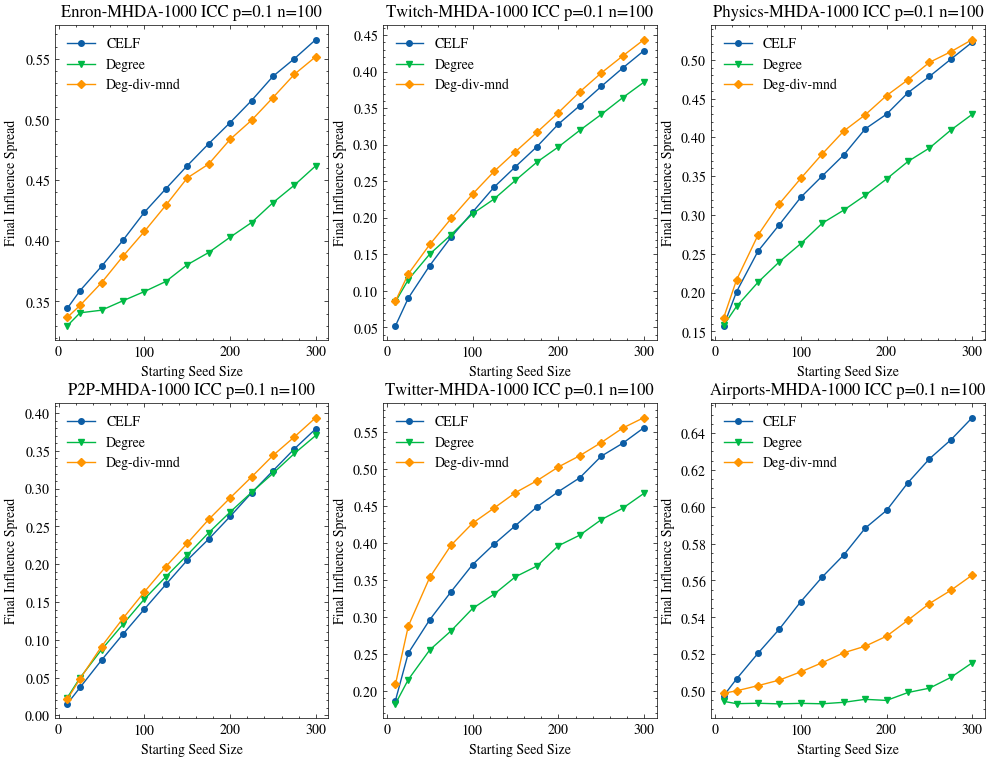
\includegraphics[width=\textwidth]{ICC p=0.1 n=100-performance.png}

		\caption{IC Performance $p=0.1$ $n=100$}
		\label{icc-p-0.1-perf}
	\end{center}
\end{figure}

As shown in figure \ref{icc-p-0.1-perf} using the IC model with $p=0.1$ each of our six networks we outperform or at least match the degree heuristic across all seed sizes.
In four of out networks we see our heuristic exceeding CELF across all seed sizes, in the Enron dataset it is slightly below the performance of CELF but still far exceeds the plain degree heuristic. The airports dataset has a significant difference in between all of the datasets, this is likely due to the nature of high degree nodes, in this case busy airports, being primarily connected to other high degree nodes. Choosing nodes which have a low mean neighbour degree allows us to capture those far out nodes compared to just the degree heuristic.

\clearpage
\subsection{LTM Analysis}

\begin{figure}[h]
	\begin{center}
		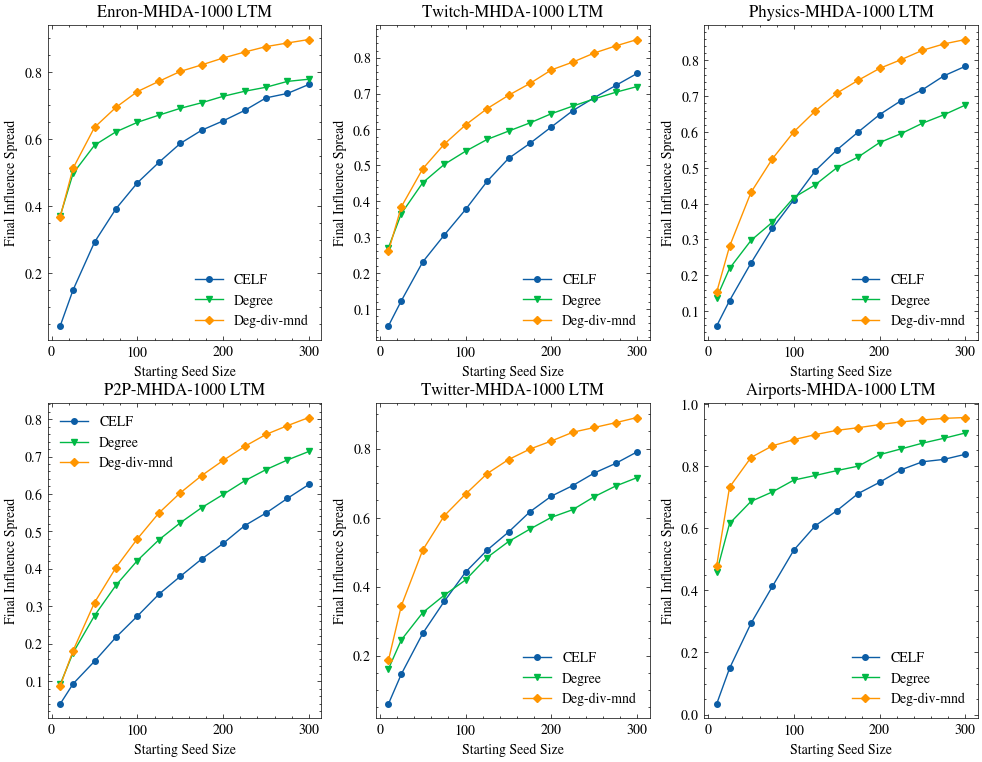
\includegraphics[width=\textwidth]{LTM-performance.png}
		\caption{LTM Hybrid Heuristics Performance $n=100$}
		\label{ltm-perf}
	\end{center}
\end{figure}

As shown in figure \ref{ltm-perf} our heuristic shows a clear performance improvement over both degree and CELF across all seed set sizes. The most interesting result is the performance of our heuristic across the linear threshold model.
\\

If we consider the initial starting state of CELF, computing a run of the model with each node on it's own then as the start point the highest degree nodes will have the greatest number of activations. During the early runs the top node is revaluated to see if it's still the best and as the first node has not spread very far it would likely be that the next best node is not a great choice either. This continues until the tipping point effect starts picking up speed and the CELF rate of growth steepens.

Activating a node $v$ it will contribute $1/\deg(u)$ towards each of it's neighbor's $u$'s activation thresholds.
For a node $u$ with a high degree this will make little change towards it activating as it requires lots of it's neighbours to tip it towards changing.
Our heuristic considers nodes with high degrees connected to lots of nodes with low degrees themselves, we are choosing seeds connected to nodes to which we can contribute the a larger proportion of their threshold, this makes them easier to activate and produces greater overall spread.
The tipping point behaviour of the threshold model is then amplified with this type of seed selection compared to CELF.

%\begin{figure}[h]
%	\centering
%	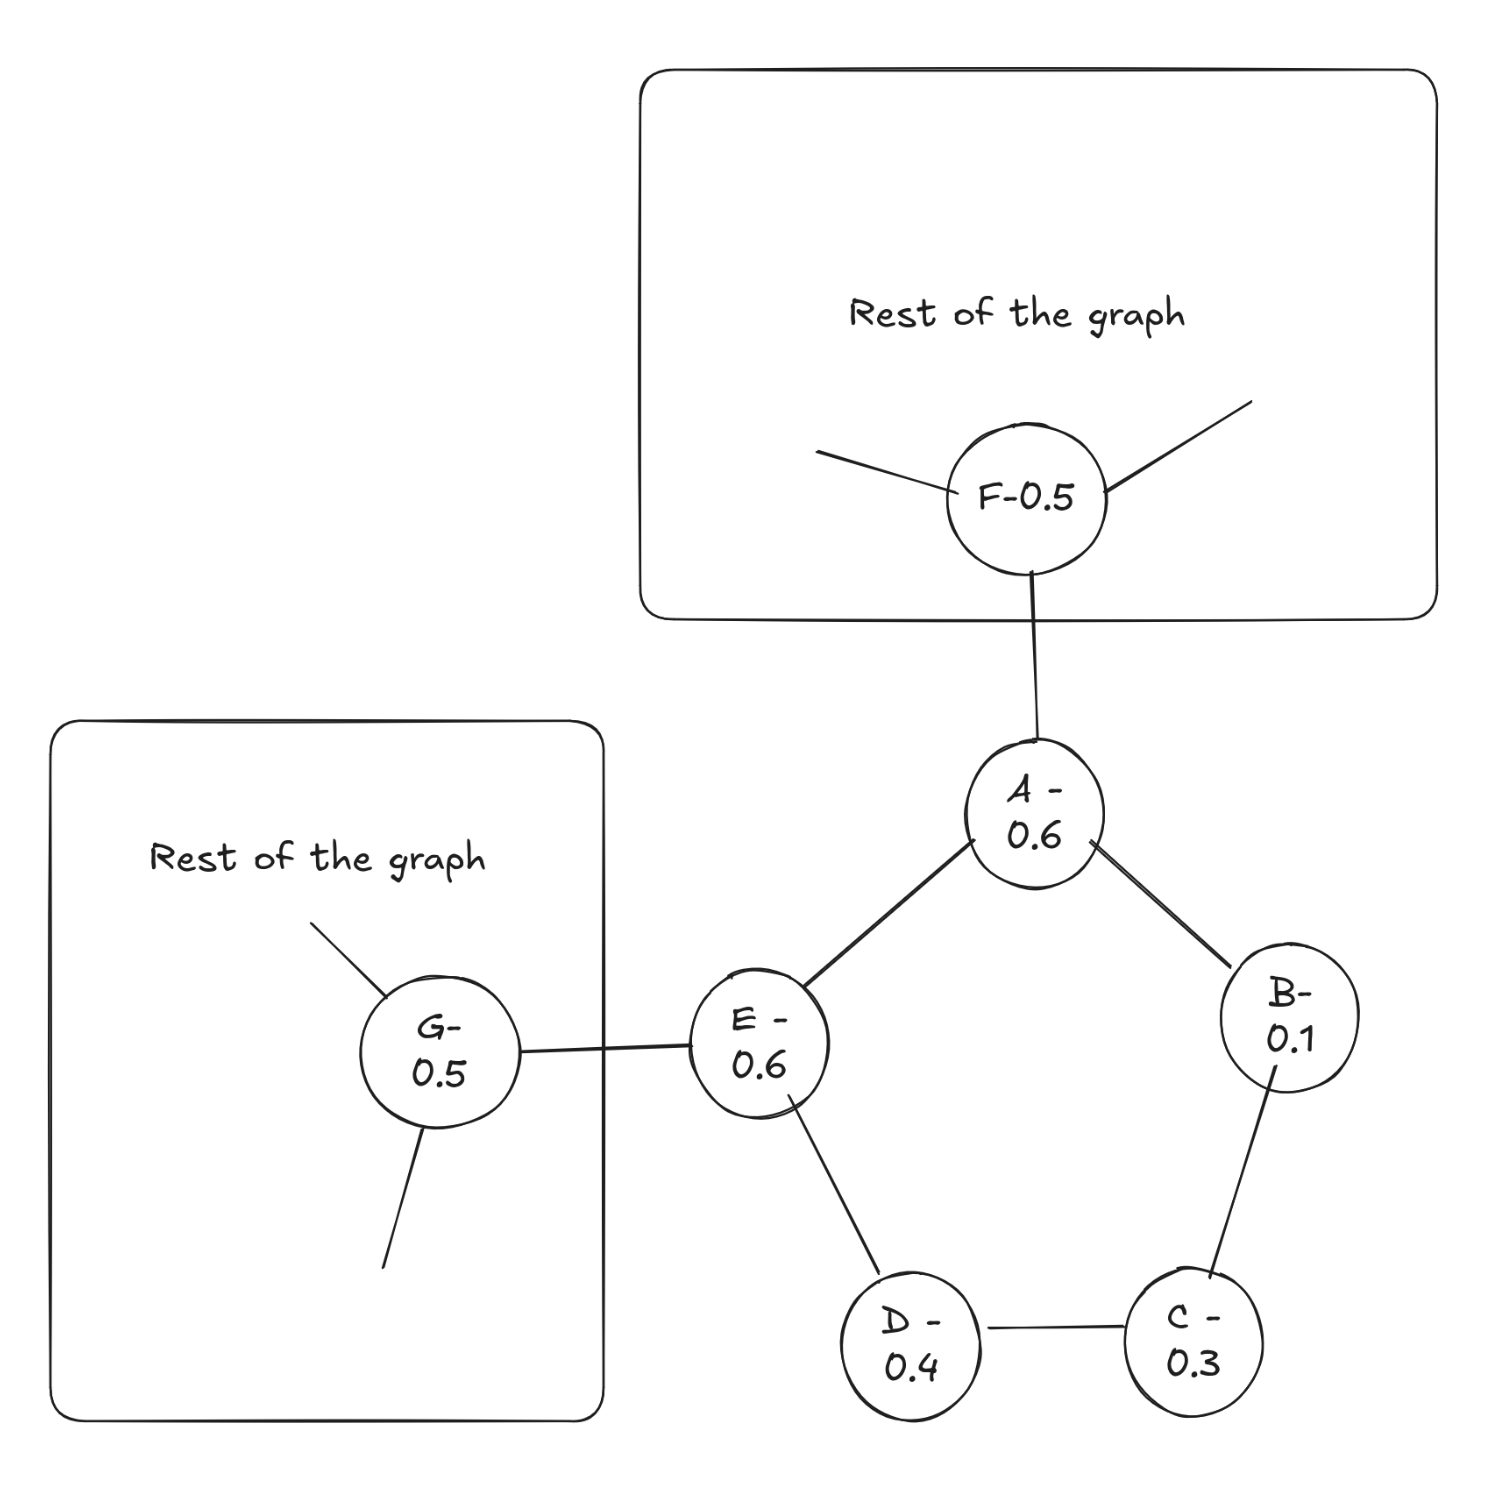
\includegraphics[width=0.8\textwidth]{Screenshot From 2026-04-09 01-59-38.png}
%	\caption{Example network for why CELF will be non optimal}
%\end{figure}

Across all of the datasets there is clear statistical evidence that at each seed size that our heuristic is a different distribution to that of the CELF distribution. Across the comparison of our heuristic and CELF produces p values in the range of $4.78 \times 10^{-134}$ an $5.72 \times 10^{-165}$ showing very clear evidence that it is a better performer across all datasets.
The minimum effect size observed is 2.27, on the Physics dataset at a seed set size of 10 nodes.

\subsection{DC Analysis}

\begin{figure}[h]
	\begin{center}
		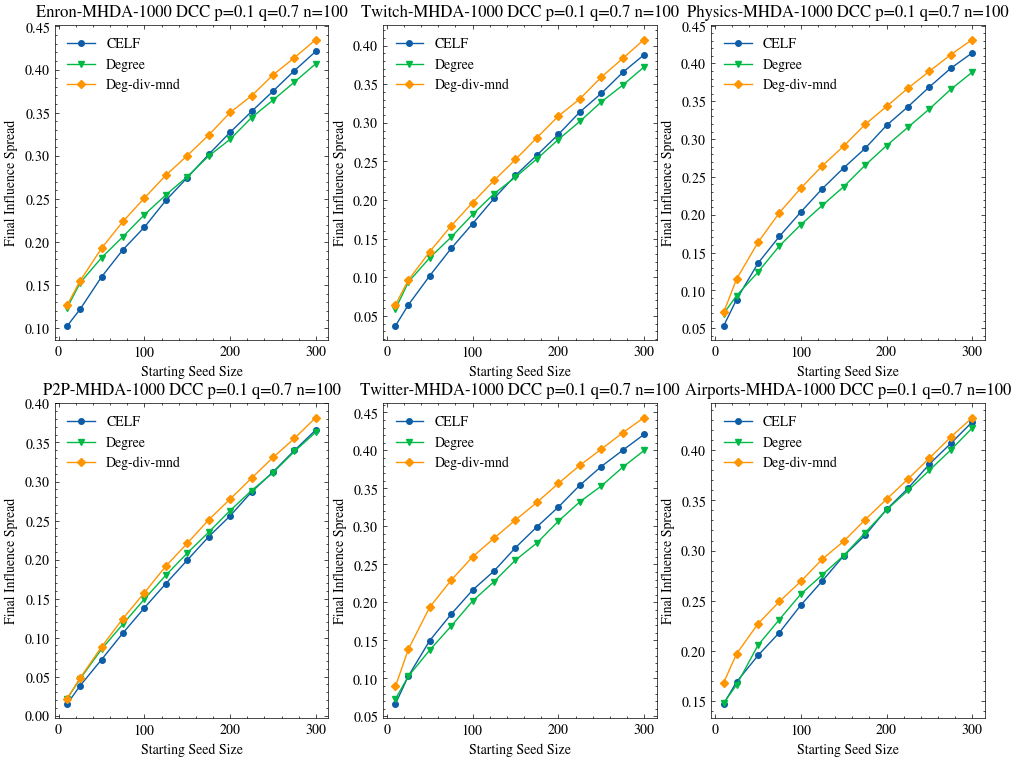
\includegraphics[width=\textwidth]{DCC p=0.1 q=0.7 n=100-performance.png}
		\caption{DC Hybrid Heuristics Performance $p=0.1$, $q=0.7$, $n=100$}
		\label{dcc-p-0.1-q-0.7-perf}
	\end{center}
\end{figure}

As seen in figure \ref{dcc-p-0.1-q-0.7-perf} our heuristic shows superior performance to both degree and CELF across the entire range of seed sizes and networks.
We see the effect of the decreasing activation probabilities decrease the effective spread of any node leading to an almost linear relationship across the range of seed sizes to the final influence spread.

Each of the graphs shows a crossover point between Degree and CELF, this is likely that as the number of seeds progresses the tendency of higher degree nodes to cluster becomes visible.
Choosing these high degree nodes as our start points each of them has attempted to influence all of their neighborhood which is now becoming harder to activate, choosing closely clustered other high degree nodes wil node be as effective as CELF which can evaluate the marginal gain of each node as it goes along and will be able to choose nodes that whilst they may have a lower degree will actually have a higher expected value for the number of nodes influenced due to having drastically higher probabilities.
Our heuristic is able to capture some of these properties of spread out nodes that are not clustered so closely together by choosing nodes attached to lots of lowe degree leaf type node.

\vspace{1em}

Across the each of the datasets we have strong evidence that our heuristic exceeeds that of CELF, p values ranging from $9.6 \times 10^{-29}$ up to a maximum of $3.9 \times 10^{-8}$ across the airports dataset which had the largest p values.
The smallest effect size observed is under the airports dataset at a seed size of 300 with a value of 0.36.
All other datasets show larger effect sizes and power analysis shows we meet the required number of runs to detect them.
We can clearly show that our heuristic outperforms CELF with statistical certainty.

\subsection{Stability across model parameters}
Finding a heuristic which works across a range of model parameters is important.
There is minimal use in a heuristic which works across a very narrow range of datasets or model parameters, being able to generalise across a range of model parameters allows to to be certain we have a good result.
We have therefore tested each of the IC and DC models with a set of parameters as listed in table \ref{param-table}

\begin{table}[h]
	\centering
	\begin{tabular}{|c|c|c|c|c|}
		\hline
		\textbf{Model} & \textbf{p} & \textbf{q} & \textbf{t} & \textbf{Reasoning}                              \\
		\hline
		IC             & 0.1        &            &            & Our Baseline                                    \\
		IC             & 0.2        &            &            & Higher variability but expect consistent        \\
		IC             & 0.3        &            &            & Even higher variability but expect consistent   \\
		\hline
		DC             & 0.1        & 0.5        &            & Much lower overall spreads                      \\
		DC             & 0.1        & 0.6        &            & Coverage of nodes becomes more valuable         \\
		DC             & 0.1        & 0.7        &            & Our Baseline                                    \\
		DC             & 0.1        & 0.8        &            & Expect to be closer to IC                       \\
		DC             & 0.1        & 0.9        &            & Expect to trend close to IC at very high counts \\
		\hline
	\end{tabular}
	\caption{Tested Parameters for Regression}
	\label{param-table}
\end{table}

Across the IC model raising values of $p$ up to 0.3 to allow for greater spread through the networks.
Higher values will introduce greater variability to the overall results, at 30 trials some of the lines oscillated around each-other due to the variance, at 100 trials they converged showing a clear separation.

Across the DC model we vary the value of $q$ in our decreasing probability function, as $q$ tends to 1 we approach the behavior of the IC mode ($q=1$ in IC), as we decrease towards 0.5 the structure of the nodes chosen becomes more important as even 2 attempts at influencing a node will drop $p$ to 0.025 making growth much slower but likely emphasizing how spread out a seed should be to be optimal.

\subsubsection{Stability of the IC model}

\begin{figure}[h]
	\begin{center}
		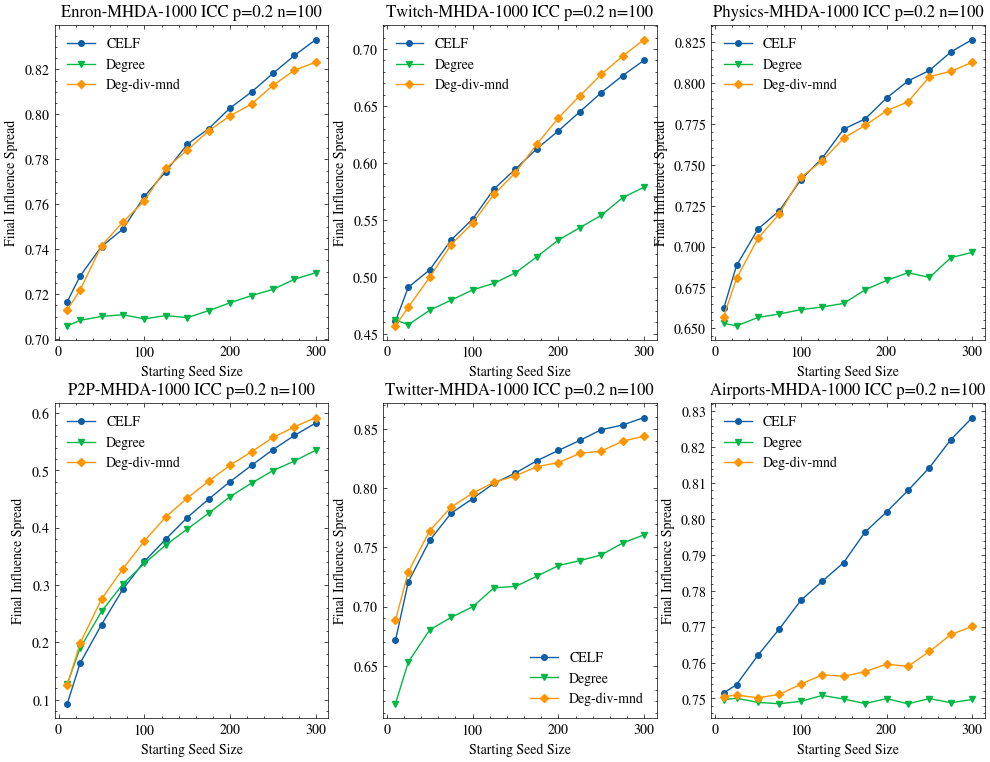
\includegraphics[width=0.8\textwidth]{ICC p=0.2 n=100-performance.png}
		\caption{IC Stability at $p=0.2$}
		\label{icc-p-0.2-q-0.7-perf}
	\end{center}
\end{figure}

\begin{figure}[h]
	\begin{center}
		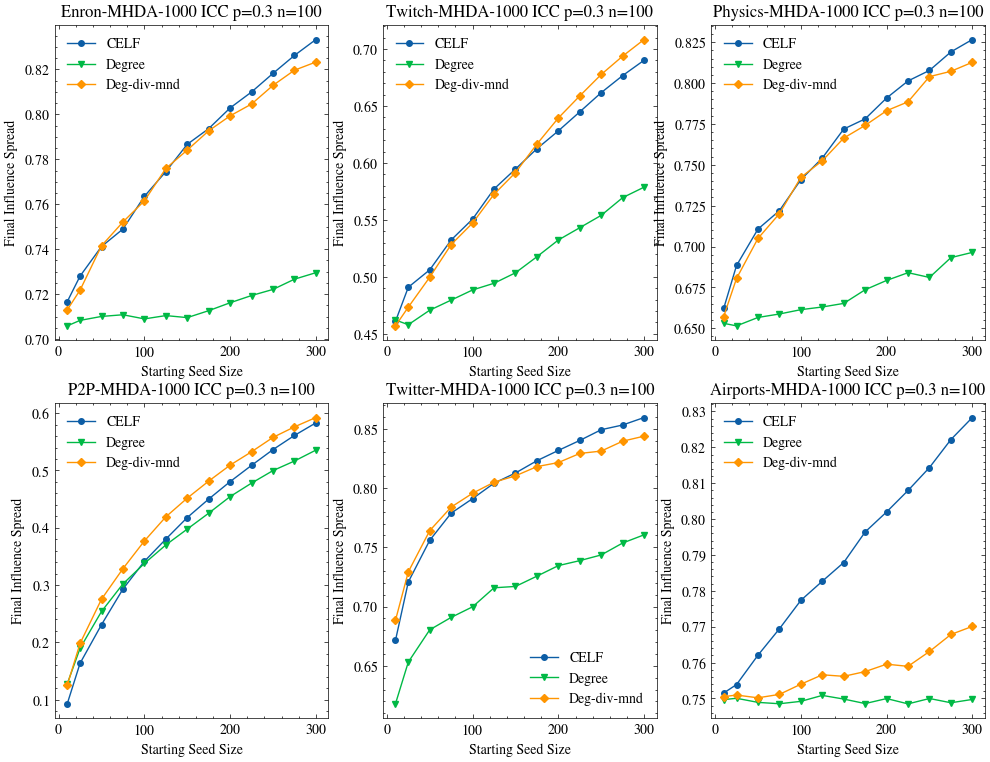
\includegraphics[width=0.8\textwidth]{ICC p=0.3 n=100-performance.png}
		\caption{IC Stability at $p=0.3$}
		\label{icc-p-0.3-q-0.7-perf}
	\end{center}
\end{figure}

Across both p=0.2 and p=0.3 the performance of our heuristic closely matches CELF until their lines cross over at around 150 seeds.
The airports dataset remains an outlier, again likely due to the very few nodes with incredibly high degrees and minimal nodes with few neighbours leading both degree and our heuristic to perform very poorly in comparison to CELF which is able to choose the best nodes based on the performance of previous nodes.


\subsubsection{Stability of Decreasing Cascde}

We show that the decreasing cascade allows our heuristic to closely match and exceed both CELF and degree across all values of q in all networks except for the airports dataset at q=0.8 and q=0.9 where they both begin to look more like the IC model which has an equivalent q=1.
The heuristic shows excellent stability and preserves it's position above the other methods across all networks except for the airports dataset.

\begin{figure}[h]
	\begin{center}
		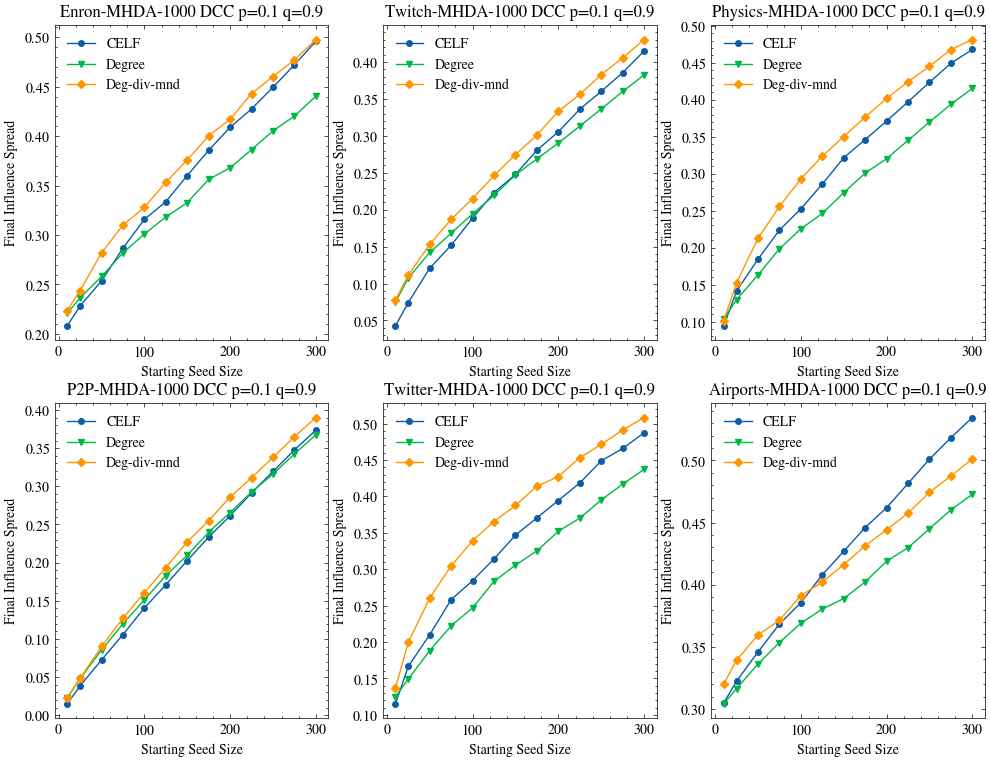
\includegraphics[width=0.8\textwidth]{DCC p=0.1 q=0.9-performance.png}
		\caption{DCC $p=0.1$ $q=0.9$}
		\label{icc-p-0.3-q-0.7-perf}
	\end{center}
\end{figure}

\begin{figure}[h]
	\begin{center}
		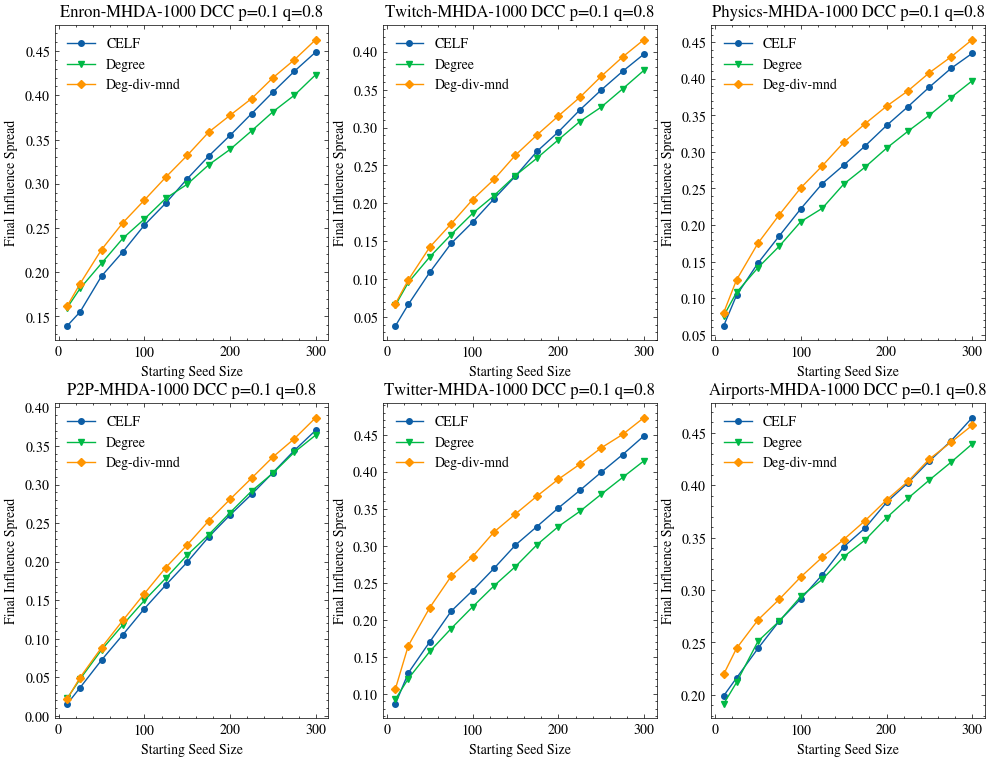
\includegraphics[width=0.8\textwidth]{DCC p=0.1 q=0.8-performance.png}
		\caption{DCC stability at $p=0.1$ $q=0.8$}
		\label{icc-p-0.2-q-0.7-perf}
	\end{center}
\end{figure}

\begin{figure}[h]
	\begin{center}
		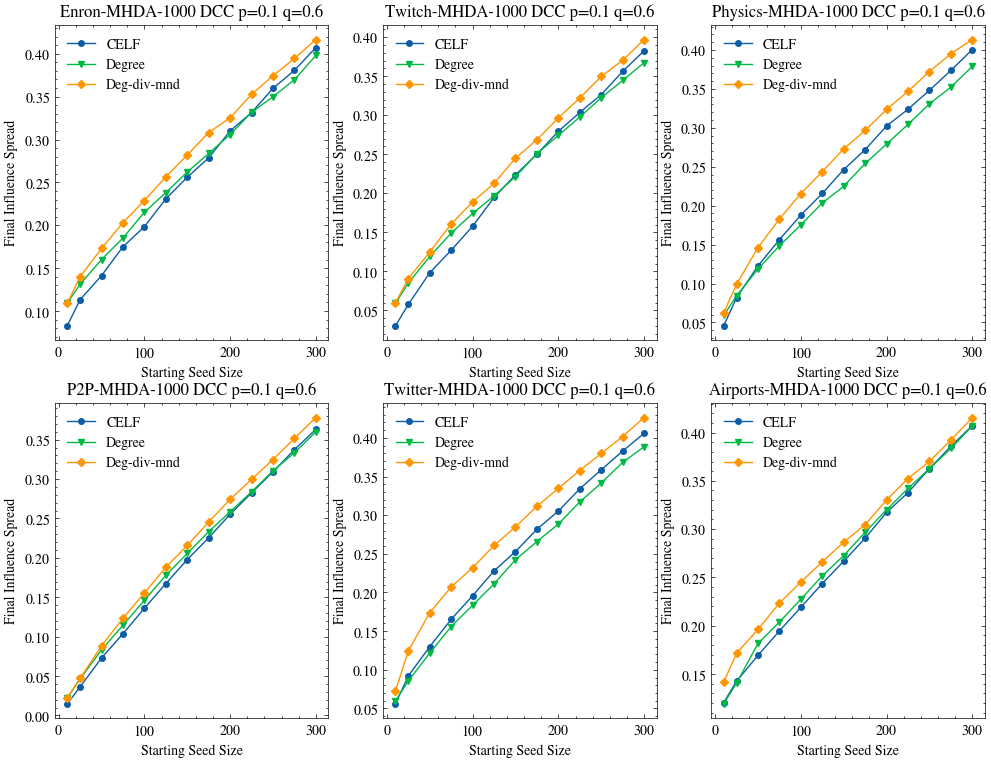
\includegraphics[width=0.8\textwidth]{DCC p=0.1 q=0.6-performance.png}
		\caption{DCC stability at $p=0.1$ $q=0.6$}
		\label{icc-p-0.2-q-0.7-perf}
	\end{center}
\end{figure}

\begin{figure}[h]
	\begin{center}
		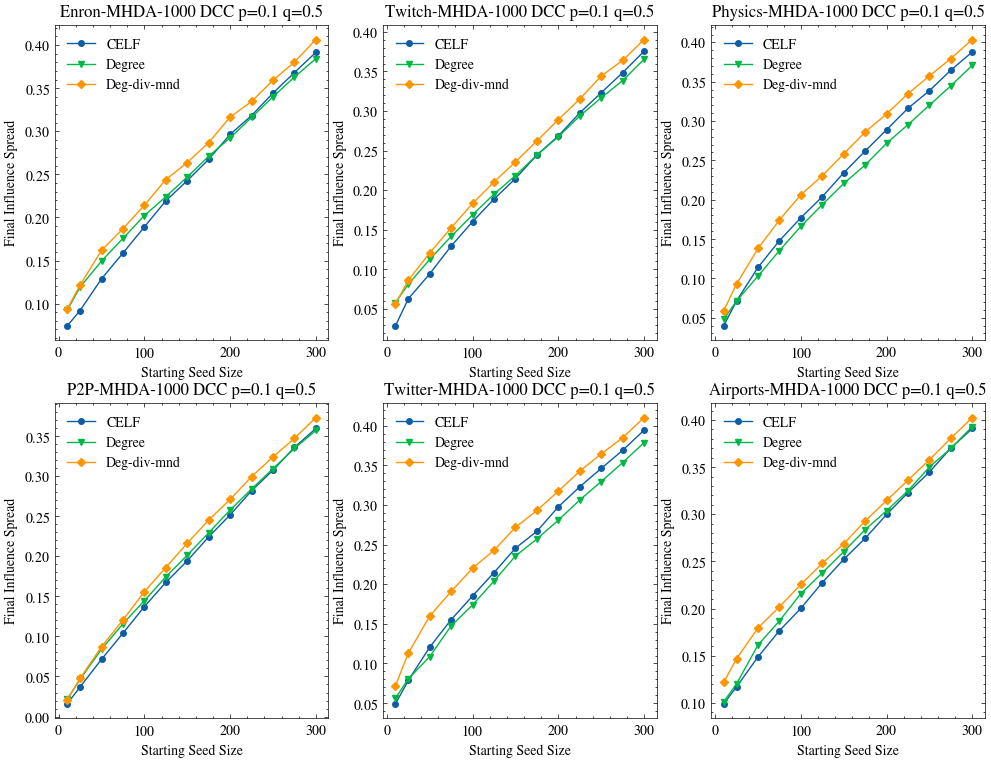
\includegraphics[width=0.8\textwidth]{DCC p=0.1 q=0.5-performance.png}
		\caption{DCC $p=0.1$ $q=0.5$}
		\label{icc-p-0.3-q-0.7-perf}
	\end{center}
\end{figure}

\subsubsection{Stability of the threshold model}
We have the ability to provide a custom weight function for the model based on each the network and specific node.
This would however transform the model into a constant threshold model. This was unfortunately out of the scope of the project at this moment however we would be keen to investigate it in the future.

\clearpage
\section{Limitations}

We have considered a range of networks covering a large number of real world topologies.
Investigation into the differences of performance across each of the models on different sampling methods.
Varying the size of the samples would be a good way of testing that the heuristics scale to generalised network sizes.
\\

Investigation into the correlation between the relationship with seeds chosen by CELF in an IC or DC scenario and how they translate into influence under the LTM model would be a very interesting area to explore.
It would be interesting to explore the relationship between the function that governs the decrease in activation probability for DC and how it correlates to the performance of the IC model with the same baseline $p$.
\\

We investigated the threshold model with unweighted edges, meaning for a node $v$ each activated neighbour contributes 1/deg(v) towards the threshold for $v$.
Investigating providing different weighting functions to allow for specification of edge weights dependant upon the network, the two nodes either side of the edge would be a good way to further understand the dynamics of the tipping point at which the network becomes quickly activated.


\clearpage
\section{Conclusion}

We have shown that for the influence maximisation problem a simple structural heuristics with no global knowledge of the network is able to outperform the greedy (1-1/e) approximation on the majority of networks and topologies.

Our heuristic scores nodes on the ratio of their degree to their neighborhood's mean degree, this chooses nodes which have a large amount of poorly connected neighbors.
This prevents the tendency of high degree nodes being clustered closely together thereby allowing us to reach distinct parts of the network.

Results across six real world networks on samples produced by the MHDA algorithm demonstrate that the performance is strongly related to the exact topology of the network at hand.
Under the decreasing cascade model the heuristic strongly outperforms both the degree heuristic and CELF across all networks.

Under the linear threshold model the heuristic delivers excellent performance across all networks, this is due to the inability of CELF to recognise groups of nodes which together may be very influential whilst individually contributing very little.

Community based methods were investigated as they are known to deliver excellent performance across a variety of networks.
However the results obtained did not show conclusions to suggest an improvement over current methods.
In the future further investigating in this direction could be an excellent extension for incorporating our new heuristic for use inside community based methods.

\newpage
\bibliography{../sources}{}
\bibliographystyle{plain}

\end{document}